% use one column style 
\onecolumn 
\begin{appendices}
\section{Background of Skin and it's Interstitial Fluid}
\label{Appendix_A}
\subsection{Background of Skin}
As the MN device needs to penetrate the skin barrier, knowledge of it is vital. Skin is the largest organ of the human body with an average surface area of two square metres in adults \cite{brown2021histology}. Skin thickness varies depending on the body part from 0.5mm thick on the eyelids (thinnest skin) to 4.0mm thick on the heels of the feet (thickest skin) \cite{brown2021histology}. Functions of the skin include protection (against UV light, mechanical, thermal and chemical stresses, dehydration and biological threats), sensation (contains receptors that sense touch, pressure, pain and temperature), thermoregulation (contains sweat glands, hair, and adipose tissue) and metabolic functions (subcutaneous adipose tissue is involved in the production of vitamin D, and triglycerides) \cite{brown2021histology}. We focus on the basic skin structure that affects the mechanical design of MN biosensors for successful penetration. Skin is composed of three layers \cite{brown2021histology,GARCIAGUZMAN2021116148}:
\begin{enumerate}
    \item The epidermis (thin outer layer): A keratinised stratified squamous epithelial layer of the skin that is important for the protective function of the skin. Its thickness varies between 50 - 150 um \cite{GARCIAGUZMAN2021116148}. It is divided into five sublayers \cite{brown2021histology} among which are the stratum corneum (SC) which is lipophilic and the stratum basale (SB) which is hydrophilic \cite{GARCIAGUZMAN2021116148}. The SC is the outer layer of the epidermis which serves as the primary barrier between the body and the environment \cite{brown2021histology}. Sc thickness is about 10um \cite{GARCIAGUZMAN2021116148}. The SB also known as stratum germinativum, is the deepest layer of the epidermis, separated from the dermis by the basement membrane (basal lamina) and attached to the basement membrane by hemidesmosomes \cite{brown2021histology}.
    \item The dermis (thicker middle layer): The connective tissue layer of skin containing collagen and elastic fibres that is important for sensation, protection and thermoregulation. The thickness of the dermis varies between approximately 500 and 2000 um \cite{GARCIAGUZMAN2021116148}. The pressure needed to penetrate this layer is about 1-5MPa \cite{smalls2006effect}. It contains nerves, blood vessels, fibroblasts, sweat glands, hair follicles (in some areas) and derma lymph nodes \cite{GARCIAGUZMAN2021116148,brown2021histology}. 
    \item The hypodermis (inner layer): The thickest of all the three layers. It contains adipose tissue, sweat glands, nerves and blood vessels. 
\end{enumerate}
\subsection{Using ISF as the source for sepsis biomarker detection}
Most of the required mechanical properties of MN biosensors (length, shape, rigidness, and thickness among others) depend on the biofluid source. Blood is considered the primary biofluid source for analysing and acquiring biochemical information. Blood composition constantly changes as the patient’s health condition changes. The dermal and hypodermal layers of the skin contain blood vessels, thus, enabling MN biosensors the ability to perform blood analysis. However, several challenges arise from performing blood analysis: 
\begin{enumerate}
    \item There are high concentrations of interfering species present in the blood resulting in severe fouling issues for the biosensors.
    \item MN biosensors are intended for continuous monitoring, hence, the device needs to provide the most painless user experience; More painless than traditional finger pricks.
\end{enumerate}
Skin ISF has similar profiles of proteins, small molecules, and RNA to blood and contains specific biomarkers that are exclusive or sufficient compared to blood as it comes into contact with tissues, cells, and blood capillaries \cite{liu2020microneedles}. It contains the biologically relevant biomarkers required for diagnosing sepsis. Furthermore, using skin ISF as the source for sepsis biomarkers could potentially address the issues of direct blood analysis. ISF is found in the subcutaneous tissue and, hence, MNs with shorter lengths can be used to access ISF translating to painless skin insertion of the MN device. This allows the possibility for minimally invasive, continuous biomarker monitoring over a period of hours to days, or even longer and provides on-body portability and wearability. In addition, it allows compatibility with the diagnosis of infants. Skin ISF as a biofluid source will dramatically reduce the problems of surface fouling due to having lower concentrations of proteins and other large molecules \cite{heikenfeld2018lab}; This facilitates long-term electrochemical readout. In conclusion, skin ISF was determined to be the ideal choice for the source of sepsis biomarkers for our MN biosensors to enable real-time continuous monitoring of sepsis biomarkers in a minimally invasive manner. 
\section{Microneedle Design}
\subsection{Microneedle Analytical performance}
The procedures and materials used for the fabrication design of the MN sensors strongly influence the final analytical performance and in vivo suitability of the MN device. Usually, solid MNs that are externally modified are used for developing MN biosensors as it facilitates good interaction with the target biomarker \cite{calio2016polymeric,bollella2019minimally}. However, upon skin penetration, the recognition element is susceptible to friction with the skin layers and exposed to undesired molecules present in the skin which could damage or change the recognition element. Potential solutions to mitigate this include: 
\begin{enumerate}
    \item Using an external water-soluble polymeric layer that protects the recognition element from mechanical alteration during skin penetration. Once it has penetrated the skin barrier, the layer dissolves in the ISF allowing for direct exposure to the target biomarker \cite{jin2019reduced}.
    \item Internal modification of hollow MNs to provide physical protection of the recognition element during insertion and reduces unwanted contact with tissues, hence, reducing the fouling effect \cite{zhao2020silk,miller2012multiplexed}.
\end{enumerate}
Regardless of the method of incorporating the recognition element into the MN, resistance to skin insertion must be evaluated before any in vivo application to ensure the analytical performance of the MN sensor is not affected by skin insertion or once inside the skin. 
Therefore, there is a need to confirm that external calibrations performed in in-vitro experiments can be used for calibrating biomarker concentrations in skin ISF. To confirm this, the MN biosensor is inserted through an agarose hydrogel that is in contact with artificial ISF to mimic the skin system in the human body \cite{bollella2019minimally}. Then, we measure and record the signals obtained from the MN device through the agarose hydrogel at increasing biomarker concentrations in artificial ISF and compare the calibration graph before and after insertion of the MN in the gel. To better mimic the skin system in the human body, we can use animal skin fixed onto a physical support which allows contact with artificial ISF where biomarker concentrations can be manually changed instead of gel. 
% ====================================================================
\subsection{Cytotoxicity Testing}
As the MN penetrates the skin barrier and comes into contact with skin ISF, it is vital to ensure that there is no toxicity effect caused by direct contact, leaching, or detachment of the recognition element \cite{GARCIAGUZMAN2021116148}. Cytotoxicity assays can be used to assess cell viability after exposure to the recognition element and/or its different components which is compared to a control group for certain lengths of time (e.g. after 24-72 hours). The effects of direct contact between the recognition element and the cells and effects of leaching/detachment of singular components to the cells can also be examined by other experimental procedures such as cell proliferation experiments. We should also study skin inflammation and immune response after MN biosensor insertion with the latter being related to the biocompatibility of the device \cite{kim2019continuous}.
\subsection{Microneedle Shape}
The 3 essential factors to consider while developing MN biosensors are: resistance
to skin penetration, the pain inflicted on the end-user, and the location of the target biofluid \cite{GARCIAGUZMAN2021116148}. When considering resistance to skin penetration, parameters such as MN length, type of material, shape, tip angle, and insertion force are studied for developing a robust device capable of reaching the SC or deeper with minimal penetration force and, therefore, provide a more painless user-expereimence. The skin epidermis and dermis at the body region of MN application must be independently evaluated to design the MN biosensor; The different mechanical properties, depths and skin viscoelasticities have to be taken into consideration for the MN design. \\\\
An ideal MN biosensor is said to have: (1) an elegant tip shape (conical) \cite{chang2020optimal} and minimised tip radius (5-80um) to minimise the insertion force required, (2) adequate MN thickness (5-60um), base diameter (100-200um) and Young's Modulus to prevent fracture and (3) adequate MN length to reach the biofluid source (below 600 um for ISF) \cite{GARCIAGUZMAN2021116148}. The length of the MN has to be long enough to reach the target biofluid by penetrating the appropriate skin layers but not be too long to cause axial fracture, thus, a compromise has to be made. Several studies have attempted to quantify the pain experienced by volunteers as a result of MNs and MN arrays. The effect of MN length, base diameter, thickness, number of MNs per array, and tip angle, have been studied \cite{li2013optimized, gill2008effect, lee2018three}; A direct correlation between the patient's pain and MN length (up to 1450 um) and the number of MNs placed (up to 50) was observed. MN arrays with varying thickness or tip angle, up to values of 100 um and 90 degrees, respectively, no change in discomfort levels were observed. Finally, every patient indicated that the discomfort caused by MNs was always less than that caused by regular hypodermic needle insertion (outer diameter of 460 um and insertion depth of 5 mm). 
\subsection{Forces experienced by Microneedles}
MN robustness, insertion force and tip fracture force were assessed in various studies \cite{davis_landis_adams_allen_prausnitz_2004, jung-hwan, römgens_bader_bouwstra_baaijens_oomens_2014} for a range of MN tip radii, lengths, geometries and wall thickness and  wall angles. Different imaging technologies can be used to precisely assess the state of the MN tips. This includes the USB camera attached microscope. To visualise the MNs tips with a higher magnification, scanning electron microscopy (Hitachi 3500, Pleasanton, CA) was used \cite{davis_landis_adams_allen_prausnitz_2004}. Different base radii are usually not tested due to the consideration that the stress maximizes on the microneedle tip \cite{formulas_stress}. Various authors have reported a linear dependence of the tip insertion force with the interfacial area of the needle tip. An increase in wall thickness, wall angle and tip radius was found to increase the force required to fracture the microneedles; This was supported by finite element simulations and a thin shell analytical model. Most studies used the change in electrical resistance of the outermost layer of the skin to determine the penetration point of the needle due to the high chance of inaccuracy of the visual assessment. Studies on the insertion force of the microneedle through the skin were reported to be in the range of 0.08 to 3.04 N,  for tip radii of 30 to 80 mm and wall thickness of 5mm \cite{davis_landis_adams_allen_prausnitz_2004}. It has also been shown that the average insertion force for hollow microneedles did not differ much from that of solid MNs; This leads to the conclusion that a full cross-sectional area is a better representation of an inserted microneedle in the skin, rather than the annular surface area. The fracture force was determined by pressing the microneedles against a test block until fracture occurred. Fracture force measurements were taken for wall thickness ranging from 5µm-15µm, tip radii of 40-58µm and wall angles of 60-70 degrees giving fracture forces values of 0.5N-6N, , 1.5N-6N and 1.2N - 3N respectively. Decreased tip radius drastically decreased insertion force and moderately decreased fracture force while increased wall thickness and wall angle drastically increased fracture force but had no effect on the insertion force over the range of MN shape considered. Thus, fracture force depend mostly on wall thickness and only slightly on tip radius and wall angle. This is supported by theoretical considerations where an increase in wall thickness, increases the area over which the force is applied and, thus, decreases the stress on the needle. In addition, as the microneedle wall angle gets more vertical and the shape of the microneedle approaches cylindrical, a higher fraction of the stress would get oriented along the plane of the wall rather than normal to the wall, thus, increasing the fracture force. Fracture forces were shown to always be greater than the insertion forces. Therefore, using MNs of small tip radius and large wall thickness could potentially result in a 5-fold margin of safety, which  is the ratio between the insertion and fracture forces. 

\subsection{Chemical Stability of Aptamers}
Microneedle Electrochemical Aptamer based biosensors introduced into the human body will unavoidably interact with human serum. Aptamers, being single stranded oligonucleotides, are susceptible to nuclease degradation in serum, thereby affecting it's function in vivo \cite{kratschmer2017effect}. RNA has a half life on the order of seconds, prolonged to minutes/hours for DNA molecules \cite{morrissey2005activity,kurreck2002design}. Chemical Modifications to the sugars such as 2’-fluoro (2’F) or 2’-amino
(2’NH2) ribose groups on the pyrimidine residues have shown to improve serum half-life \cite{barciszewski2009locked}. Stabilizing backbone modifications can
also be incorporated into aptamers by substituting backbone phosphate linkages (PO) with sulfur-containing phosphorothioate
linkages (PS) \cite{green1995nuclease} and phosphorodiothioate linkages \cite{yang2004progress}. In addition to sugar and phosphate modifications, the 3’ end of the molecules are usually capped with an inverted
dT residue, which provides resistance to serum exonucleases \cite{dass2002cellular}.\\\\
 Serum stability is a critical feature for assessing the viability of this sensing platform for preclinical in vivo studies, however there have been a lack of comprehensive and systematic studies of the effect of composition
 on aptamer serum stability.

\newpage
\section{Nitrite Sensor Protocol} \label{app:nitrite_protocol}
\textbf{Adopted from} Electrochemical Biosensors, Raphaël Trouillon (2011), Imperial College London\\ \textbf{Prepared by} Peter Xie, James Tang, Safiyya Musa \quad  \textbf{Reviewed by} James Mcleod, Shulin Zhang
\subsection{Electrochemical Detection of Nitrite Investigations} 
\textit{Aim: To Establish baseline ability of electrode to sense nitrite in ideal conditions, between concentrations of 4-20$\mu$M (Nitrite in PBS). Serum nitrite concentrations in healthy individuals is around 1.7 $\mu$M, whereas patients infected with sepsis have higher concentrations.} \\\\
Nitrite Investigation Summary:
Differential Pulse Voltammetry (DPV) on nitrite solutions performed using the apparatus setup in Figure 1 with a 2 mm gold electrode (CHI101) as the working electrode (WE), platinum wire (CHI115) as the counter electrode (CE) and Ag/AgCl electrode (CHI111) as the reference electrode (RE). The blank electrolyte was pH 7.4 phosphate – buffered saline (PBS). The WE were polished with alumina slurry. WE is then washed with deionised water and sonicated in ethanol. DPV was performed using the PalmSens Emstat3 potentiostat with default parameters adjusted experimentally for performance.
\subsection{Reusable Gold Electrode Cleaning (Essential between Experiments)}
\begin{enumerate}
    \item Place three MicroCloth polishing pads (Buehler) into three Petri dishes
    \item Use spatula to place 1.0 $\mu$m, 0.3 $\mu$m and 0.05 $\mu$m dry alumina (Buehler) into the three plates, respectively
    \item Add distilled water to form alumina slurries
    \item Starting with the 1.0 $\mu$m plate and decreasing in size, move the 2 mm gold working electrode (CHI101) through the slurry in a figure-eight pattern, with the electrode perpendicular to the surface of the plate, and wash the electrode with deionised water after every polishing
    \item Place electrode into a bottle with 5\% ethanol and deionised water
    \item Insert bottle into VWR ultrasonic cleaning bath for 5 minutes
\end{enumerate}

\subsection{Production of Phosphate buffered solution (PBS)}
\begin{table}[H]
    \centering
    \begin{tabular}{|c|c|}
    \hline
    \textbf{Reagent} & \textbf{Mass(g)}  \\ 
    \hline
    NaCl & 8.0 \\
    KCl & 0.2 \\
    Na\textsubscript{2}HPO\textsubscript{4} & 1.44 \\
    KH\textsubscript{2}HPO\textsubscript{4} & 0.24 \\
    \hline
    \end{tabular}
 
    \label{tab:my_label}
\end{table}

To 800ml deionised water add reagents listed above. 
Confirm with pH probe that solution is pH 7.4. Adjust with HCl if necessary.
\\
Top up with deionised water to 1L.

\subsection{Preparation of Electrochemical cell}
\begin{enumerate}
    \item Circuit Wiring and Connection: • Red – working electrode • Blue – reference electrode • Black – counter electrode • Green – ground
    \item Insert 15 mL of PBS into electrochemical cell
    \item Connect nitrogen canister to bottle of 1 M KCl solution and connect bottle to cell in order to degas the PBS
    \item Rinse Ag/AgCl reference electrode (CHI111) and platinum wire counter\\ electrode (CHI115) in deionised water 
    \item Place all three electrodes into cell as shown above
    \item Connect the Palmsens potentiostat to the electrodes via crocodile clips
    \item Perform Differential pulse voltammetry
\end{enumerate}

\begin{figure}[H]
\centering
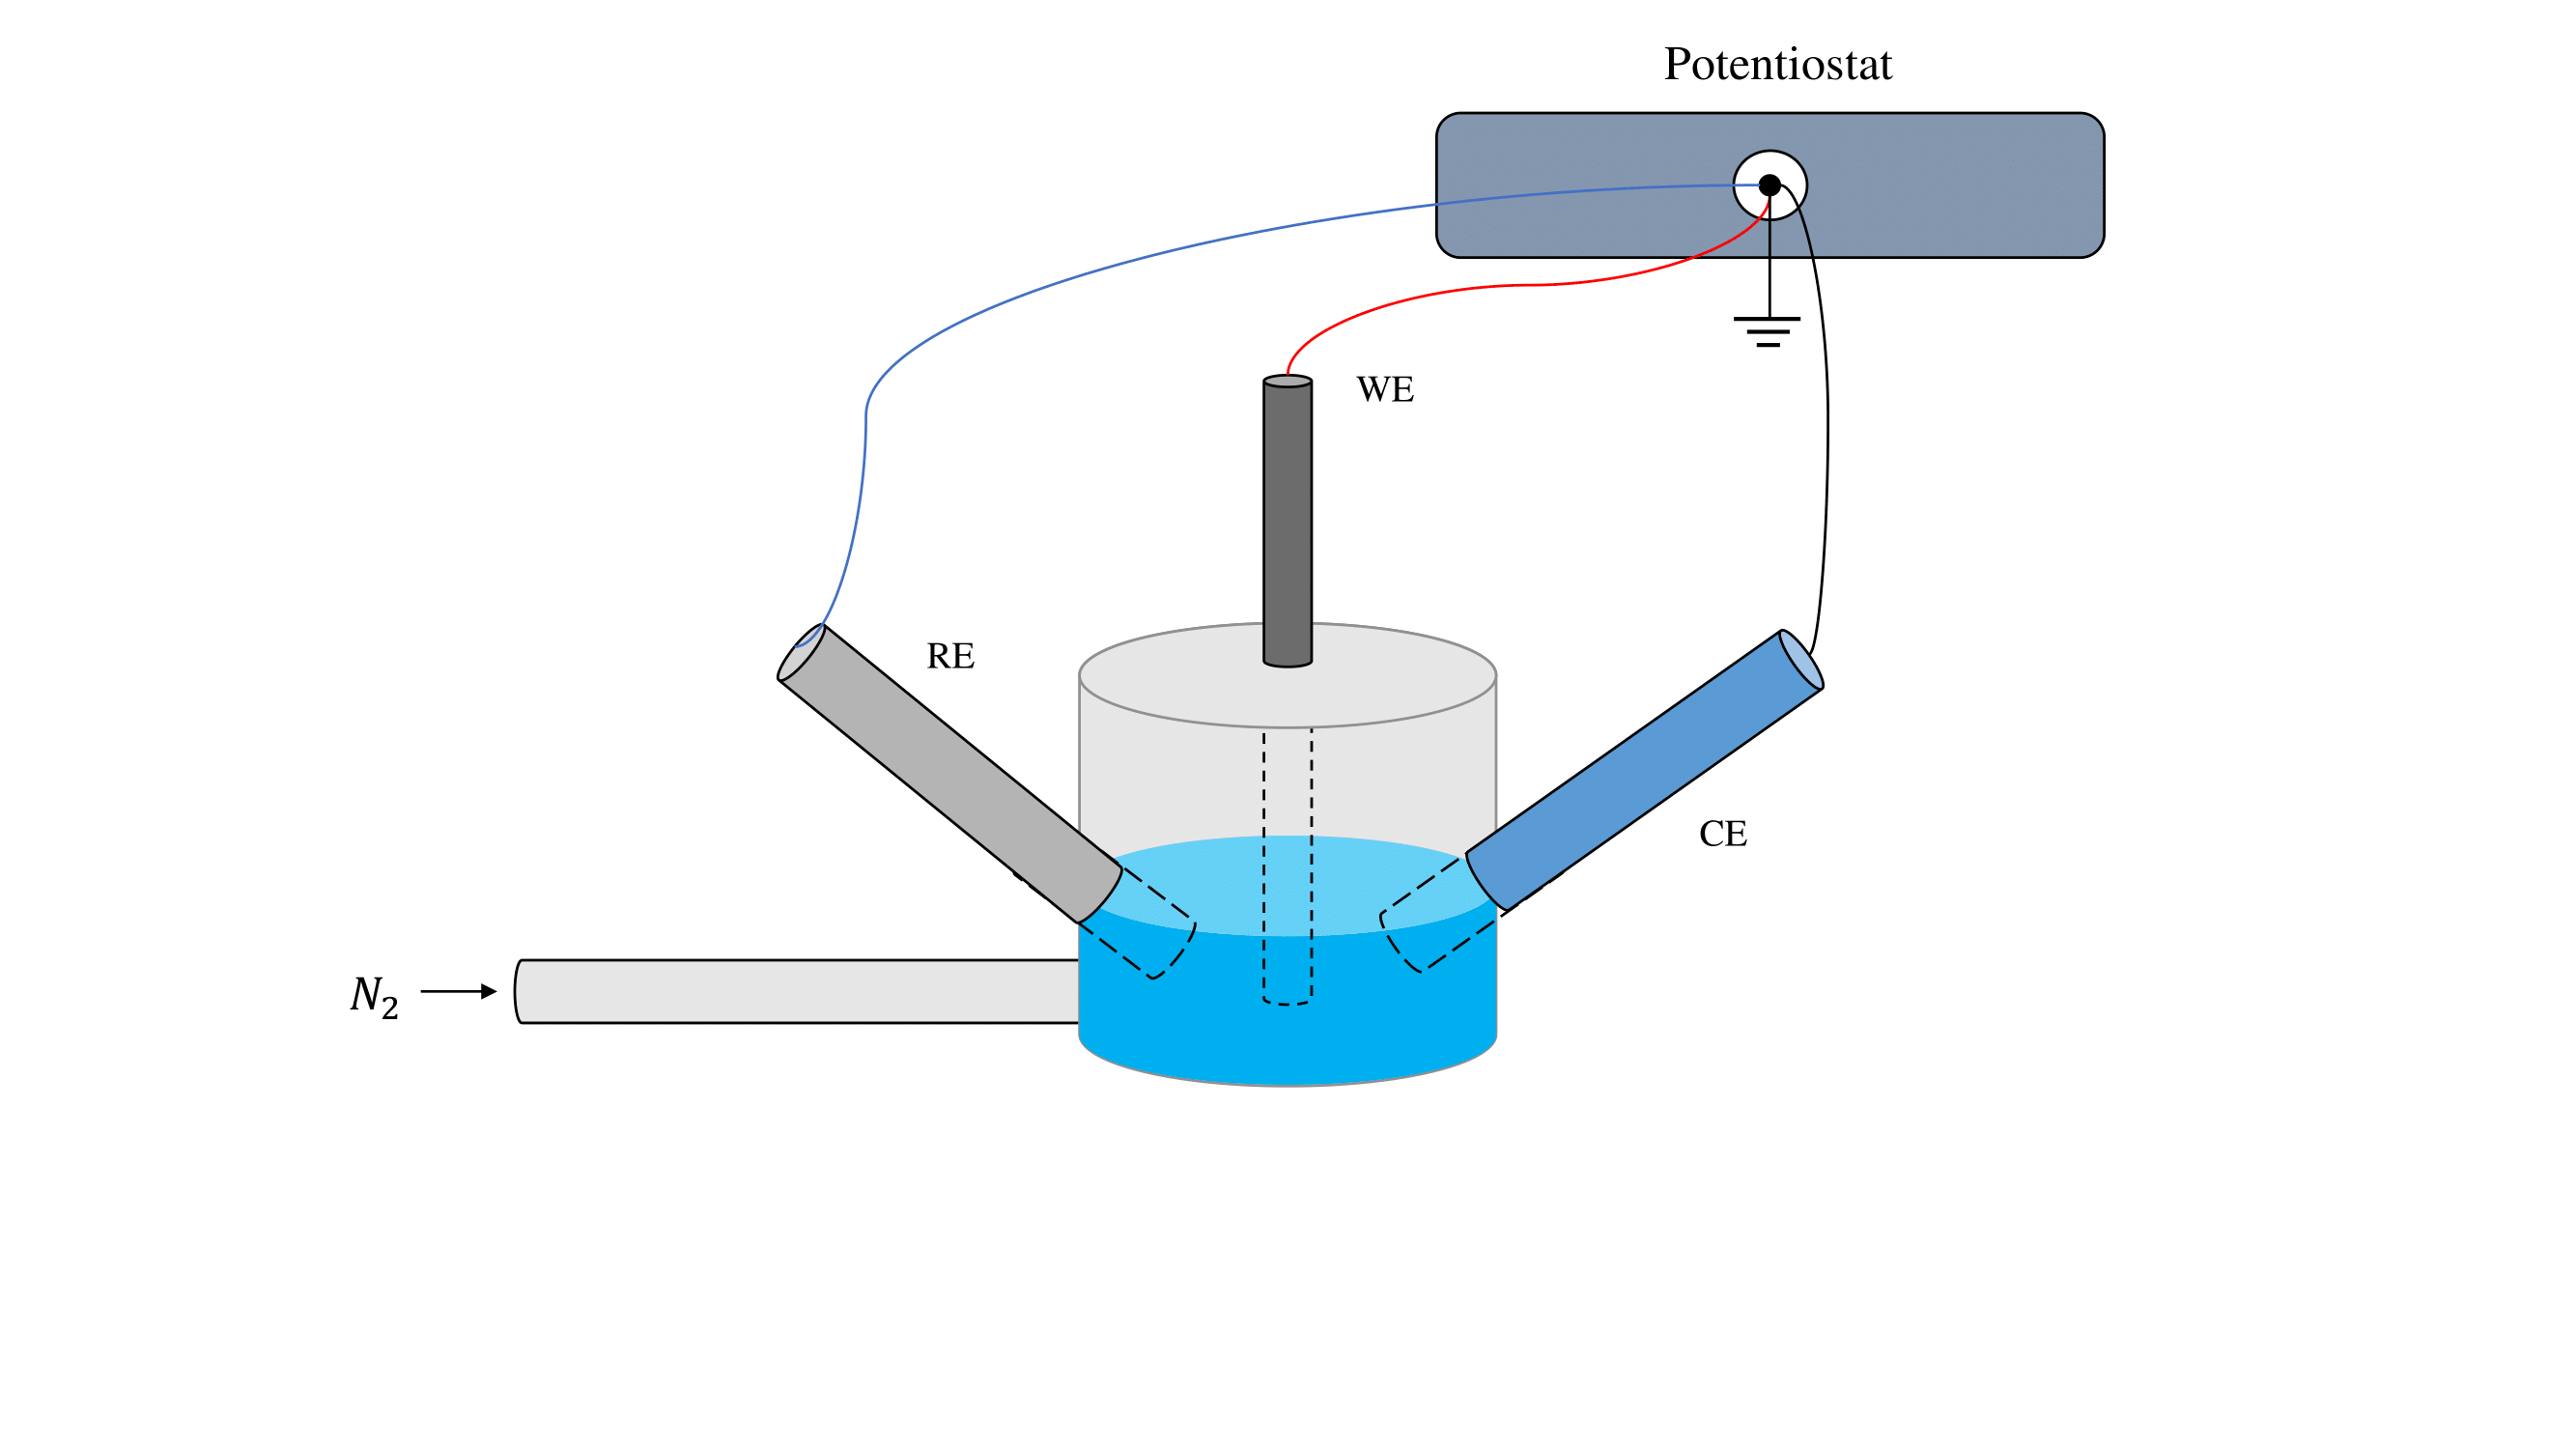
\includegraphics[height=6cm]{img/james1.png}
 \end{figure}
\textbf{Parameters for Palmsens Emstat\textsubscript{3} DPV}

\begin{table}[H]
    \centering
    \begin{tabular}{|c|c|}
    \hline
    \textbf{Parameter} & \textbf{Value}  \\ 
    \hline
    T equilibrium (s) & 10.0 \\
    Initial E (V) & 0.00 \\
    Final E (V)& 1.00 \\
    E step (V) & 0.001 \\
    E pulse/Amplitude (V) & 0.01 \\
    T pulse (V) & 0.2 \\
    Scan rate (V/s) & 0.0025 \\
    \hline
    \end{tabular}
 
    \label{tab:my_label}
\end{table}

\subsection{Production of calibration curve}

\begin{enumerate}
    \item Dissolve 17.25mg of sodium nitrite into 50 mL of PBS to produce a 10 mM sodium nitrite solution: 
    \item Run a blank DPV (run DPV without placing any of the sodium nitrite solution). 
    \item Repeat assembly of electrochemical cell a further five times pipetting 12 $\mu L$ volumes of the above sodium nitrite solution into the cell each time to give nitrite concentrations of 4 $\mu$M, 8 $\mu$M, 12 $\mu$M, 16 $\mu$M, 20 $\mu$M, 24 $\mu$M, 28 $\mu$M, 48 $\mu$M, 96$\mu$M 
    \item Perform Differential pulse voltammetry
    \item Add Sulfamic Acid, twice the number of moles as there is nitrite in the final solution, to add in excess (sulfamic acid reacts with nitrite in a 1:1 reaction).  
    \item Measure the pH of the electrochemical cell solution, and add NaOH until the pH reequilibrates to 7.4 
    \item Repeat the DPV with the original settings and investigate any changes in peak height 
    \item Construct a calibration curve by plotting peak current vs concentration of nitrite 
    
\end{enumerate}

\subsection{Albumin interference investigation}

\begin{enumerate}
    \item  Place 5.2 g of Bovine serum albumin (BSA) into a graduated bottle and add PBS until the volume inside the bottle reaches 100 mL to give a Bovine serum albumin (BSA) concentration of 52mg/ml. 
    \item Repeat Step 2 of the protocol described in Nitrite calibration curve 
    \item Construct a standard addition curve and calculate the SD and limits of detection 
    
\end{enumerate}
\subsection{Disposable gold electrode investigation}
\begin{enumerate}
    \item Wash disposable gold electrode in 75\% ethanol
    \item Produce a 15\% pHEMA solution by dissolving 250mg pHEMA in 5ml of methanol
    
    \item Add 1 drop of PDADMAC to Reference electrode and bake in oven for 1 hour at 70\textdegree{C}
    \item Add 5$\mu$L of pHEMA to Reference electrode and bake in oven for 1 hour at 70\textdegree{C}
    \item Perform Differential pulse voltammetry using the method described in nitrite investigations using the same parameters and custom testing device. Pipette solution in smaller volumes so that all electrodes are covered by the solution. Replace electrode after each DPV experiment
\end{enumerate}

%=====================================================================================
\newpage
\section{Nitrite Processing Code} \label{app:nitrite_code}
\lstinputlisting{Code/PlottingCyclicVoltammograms.m}
\lstinputlisting{Code/Plot_Calibrations_together.m}
\lstinputlisting{Code/GeneralLinearFit.m}

%=====================================================================================
\newpage
\section{Hydrogen Peroxide Electrochemical Detection Protocol} \label{app:h2o2_protocol}
\textbf{Adopted from} \href{https://pubs.rsc.org/en/content/articlelanding/2020/an/c9an02438g}{\textit{Chen and O'Hare (2020)}} \quad \textbf{Prepared by} Binghuan Li, Safiyya Musa \quad  \textbf{Reviewed by} Shulin Zhang
\subsection{PEDOT:PSS-PB Synthesis}
\textit{Aim: prepare PEDOT:PSS-PB-EG-DVS complex. Coat the working electrode with the  PEDOT:PSS-PB-EG-DVS complex.}
\begin{enumerate}
    \item Dissolve 0.03487 g ferric chloride solution in 2ml of de-ionised water (DW).
    \item 	Add PEDOT:PSS (5 ml, 0.8 wt\% PSS 43 mM PSS (monomer)) dropwise into the ferric chloride solution.
    \item Stir the solution for 2 hours, centrifuge and wash in DW twice at 8000 rpm for 10 mins.
    \item Add 20 ml (0.1 M) aqueous potassium ferrocyanide solution to the PEDOT:PSS solution.
    \item Stir the solutions for 15 minutes, centrifuge and wash in DW for three times at 8000 rpm for 10 minutes.
    \item Add 30 ml DW to disperse PEDOT:PSS.
    \item Add 20\% v/v Ethylene glycol (EG) and 10\% v/v divinyl sulfone (DVS) to the PEDOT:PSS-PB mixture to increase the mechanical stability.
    \item Apply 1.6 ul PEDOT:PSS-PB-EG-DVS on a gold working electrode (diameter 2mm). Cure in an oven at 110\textsuperscript{$\circ$}C for 1 hour.
\end{enumerate}
\subsection{Hydrogen Peroxide Solution Preparation}
\textit{Aim: set the hydrogen peroxide concentration range from 50 uM to 300 uM.}
\begin{enumerate}
    \item Dilute 9.79 M hydrogen peroxide 
    solution to 0.1 M.
    \[M_{1}V_{1} = M_{2}V_{2}\]
    \begin{itemize}
        \item $M_1$: 9.79 M, the concentration of hydrogen peroxide solution before dilution.
        \item $V_1$: 10.2 ul, the volume of the hydrogen peroxide solution before dilution.
        \item $M_2$: 0.1 M, the concentration of the hydrogen peroxide solution after dilution.
        \item $V_2$: 1 ml, the volume of the hydrogen peroxide solution after dilution.
    \end{itemize}
    
    \item Dilute 0.1 M hydrogen peroxide solution to the desired concentration.
    \begin{table}[H]
        \centering
        \begin{tabular}{|c|c|c|c|} \hline
            $M_{1}$ / uM & $V_{1}$ / ml & $M_{2}$ / M & $V_{2}$ / ul \\ \hline
            50  & 20 & 0.1 & 10 \\ \hline
            100 & 20 & 0.1 & 20 \\ \hline
            150 & 20 & 0.1 & 30 \\ \hline
            200 & 20 & 0.1 & 40 \\ \hline
            250 & 20 & 0.1 & 50 \\ \hline
            300 & 20 & 0.1 & 60 \\ \hline
        \end{tabular}
        \caption{Hydrogen peroxide concentration calculation}
        \label{tab:my_label}
    \end{table}
\end{enumerate}

\subsection{Experimental Setup}
\begin{figure}[H]
    \centering
    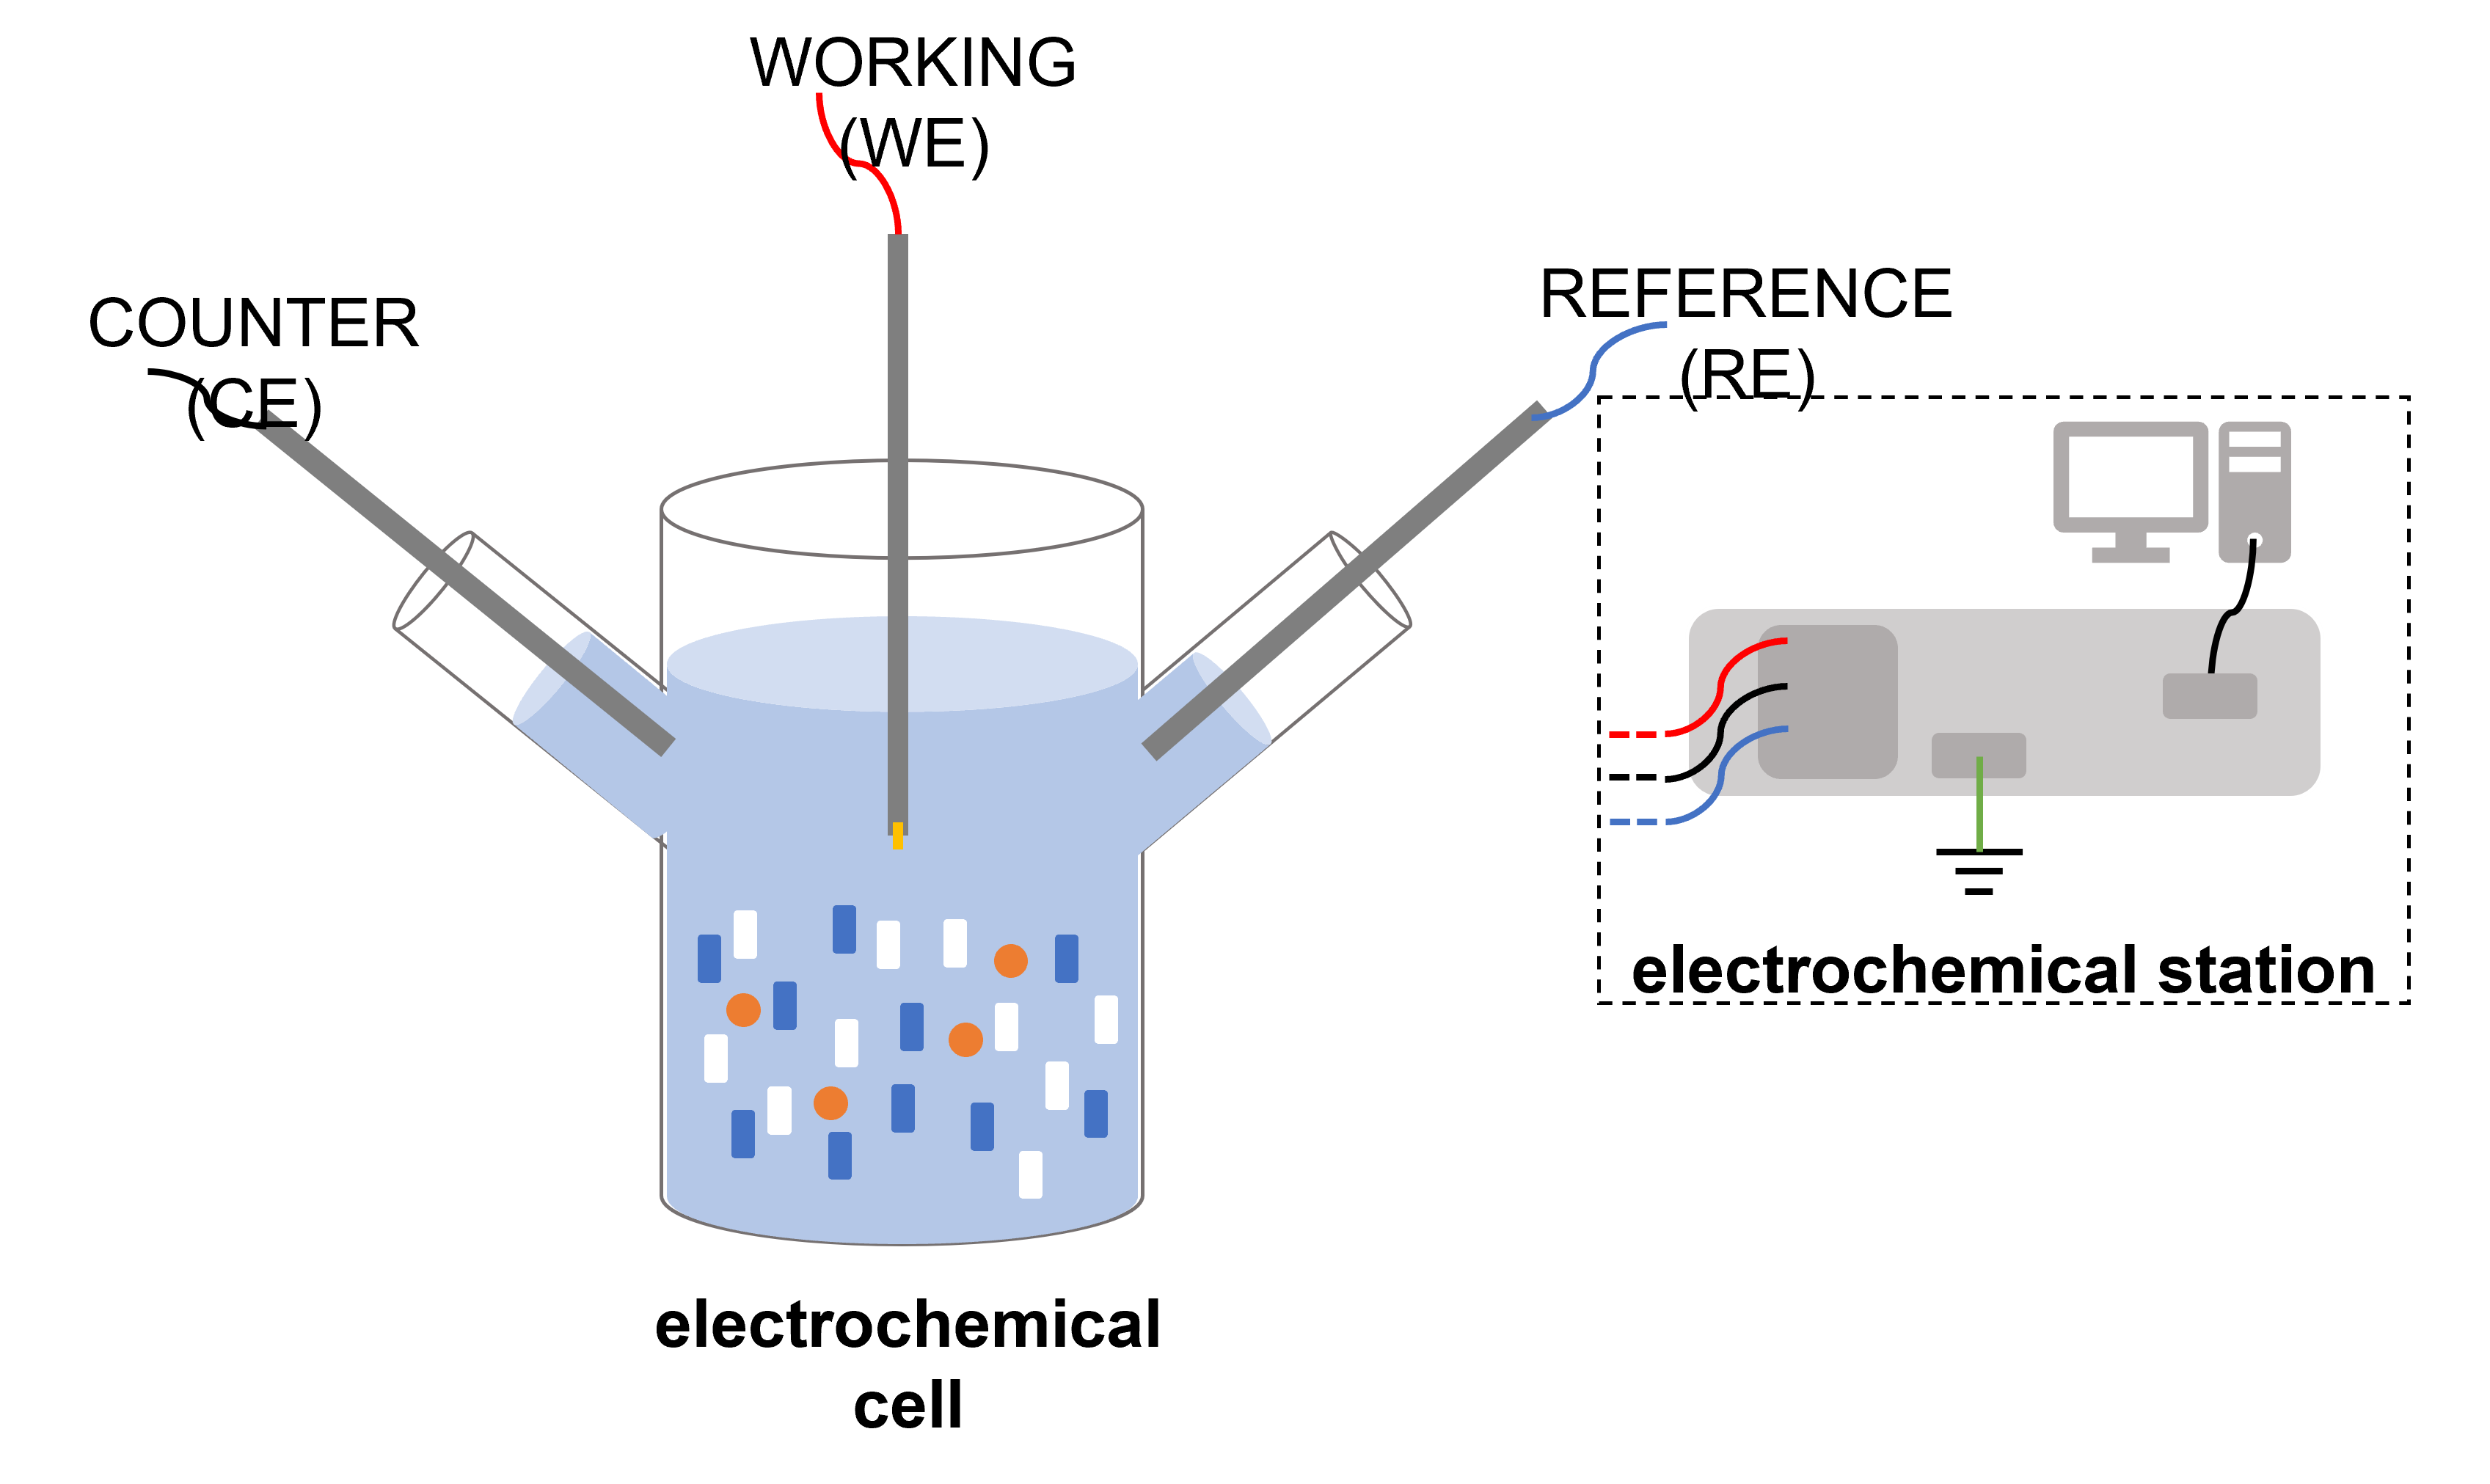
\includegraphics[width=.6\textwidth]{img/h2o2_setup.png}
\end{figure}

\subsection{Cyclic Voltammetry}
In IviumSoft\textsuperscript{\copyright}, run cyclic voltammetry  scanning in a blank buffer for 4 cycles. A starting voltage at 0.5V and an ending voltage at -0.5V  with a step increment at 1mV is applied to all scans. Scan rate is set to 100 mV/s. A stable reading is taken from the third / fourth scan. 

\subsection{Chrono Amperometry}
In IviumSoft\textsuperscript{\copyright}, run chrono amperometry scanning under each hydrogen peroxide concentration. Interval time is set to 0.03s and current range is set to 100 uA. The voltage applied to the reaction environment is set to 0.05V.

\begin{enumerate}
    \item Start the chrono amperometry scanning with the blank buffer, Waiting the data reach a stable state, pause the scanning process. 
    \item Add 10ul hydrogen peroxide solution to the buffer. Use a plastic dropper to well mix the solution.
    \item Restart the scanning. Waiting the data to be stable, pause the sampling process. 
    \item Repeat step (2) and (3) for each concentration until the concentration reaches 300 uM.
\end{enumerate} 
\subsection{Electrode Cleaning}
\begin{enumerate}
    \item Use alumina to polish the electrode (1mm, 0.3mm, 0.05mm) for 100 cycles, until no scratch can be observed on the electrode sensor surface.
    \item Rinse the electrode in de-ionised water (DIW) and clean with ultrasonic machine for 5 minutes. 
    \item No need to store in fridge.
\end{enumerate}

%=====================================================================================
\newpage
\section{Hydrogen Peroxide Coulometry} \label{app:h2o2_coulometry}
\noindent Coulometry serves as a powerful tool to amplify the signal as well as reduce the noise through integrating the amperometry current data with respect to time. By Anson equation \cite{Anson1966}, the charge can be expressed as an integral of current, as shown in \autoref{eqn:anson}. 
\begin{equation}\label{eqn:anson}
    Q(t) = \int_{t_{1}}^{t_{2}}i(t) \mathrm{d}t = \frac{nFA\sqrt{D}\sqrt{t}}{\sqrt{r}}C_{\infty}
\end{equation}
where $n$ is the number of charge transferred in the reaction, $D$ is the diffusion coefficient, $r$ is the radius of the working electrode and $A$ is the area of the working electrode.\\\\
Based on Anson equation, an improved Anson equation was proposed by Flanagan \textit{et al} \cite{Flanagan1973} by considering the edge-effect in the experiment, shown in \autoref{eqn:improved_anson}.
\begin{equation}\label{eqn:improved_anson}
    Q(t) = \frac{nFA\sqrt{D}}{\sqrt{\pi}}C_{A}\bigg( \sqrt{t}+\frac{1.92\sqrt{D}}{r}t\bigg)
\end{equation}
\noindent The realisation of coulometry is shown in the listing below.
\lstinputlisting{Code/coulometry.m}

%=====================================================================================
\newpage
\section{Lactate Sensor Protocol}
\label{app:lactate_protocol}
\textbf{Prepared by} Saylee Jangne, Safiyya Musa

\subsection{Fabrication of lactate electrode}	
\begin{enumerate}
    \item Deposit platinum black on gold electrode
        \begin{enumerate}
            \item Produce a solution of 3$\%$ w/v chloroplatinic acid and 0.005$\%$ w/v lead acetate in deionised water
            \item Apply constant current of -15 mA/cm2 for 60 s under constant stirring (vs Ag|AgCl RE and large surface area CE)
            \item Rinse thoroughly and keep wet at all times
            \item Stabilise nanoparticles by cycling in 0.5 M sulphuric acid:
                \begin{itemize}
                    \item 90 cycles -0.2 – 1.3 V at 0.1 V/s
                    \item 10 cycles -0.25 – 1.3 V at 0.05 V/s
                \end{itemize}
        \end{enumerate}
        
    \item Electropolymerisation of m-phenylenediamine (interference exclusion layer)
        \begin{enumerate}
            \item Produce a solution of 100 mM mPD in 10 mM PBS 
            \item Apply 0 V for 20 s, 0.7 V for 20 min and 0 V for 5 min (vs Ag|AgCl RE)
            \item Rinse with deionised water
        \end{enumerate}
        
    \item Coat with enzyme hydrogel
        \begin{enumerate}
            \item In 10mM of pH 7.4 PBS solution add 
                \begin{itemize}
                    \item 60 mg/ml lactate oxidase
                    \item 30 mg/ml bovine serum albumin
                    \item 2$\%$ glycerol
                    \item 60 mg/ml polyethylene glycol diglycidyl ether
                \end{itemize}
            \item Drop 4ul solution onto the electrode and after 3 mins remove 2ul
            \item Dry the sensors facing upwpards to achieve a thin film
            \item Bake in oven at 55\textsuperscript{$\circ$}C for 2 hours
        \end{enumerate}
        
    \item Coat with nafion to extend dynamic range
        \begin{enumerate}
            \item Coat electrodes with 5$\%$ solution Nafion
            \item Dry in air
        \end{enumerate}
\end{enumerate}

\subsection{Lactate Calibration Protocol}

\begin{enumerate}
    \item Electrochemical cell setup
        \begin{enumerate}
            \item Take the lactate sensor out of the freezer and hydrate by pipetting a drop of PBS on to the surface of the exposed electrode.
            \item Set up the electrochemical cell as per the diagram, ensuring the platinum and silver electrodes are in place.
            \item Add 20ml of pH 7.4 PBS to the cell 
            \item Screw the lactate sensor in to the RDE machine and suspend in solution.
            \item Connect wires to CHI potentiostat and turn the program on 0.7V for a 3 hour cycle.
            \item Turn the RDE machine on to rotate the electrode at 400rpm
            \item Allow an hour for the sensor readings to stabilise
        \end{enumerate}
        
    \item Production of lactate stock solution
        \begin{enumerate}
            \item To produce a 100mM/L solution of sodium lactate in PBS, measure 224.12mg of the sodium lactate with a weighing scale
            \item Add the lactate to 20ml of pH 7.4 PBS solution and stir gently
        \end{enumerate}
    
    \item Calibration
        \begin{enumerate}
            \item One the readings have stabilised, pipette 20uL of the lactate stock solution into the cell and record the time added- the step corresponds to the addition of 0.2mM/L lactate.
            \item Once the reading after the step has stabilised, add another 20uL
            \item Repeat the process until a concentration of 3mM/L has been reached
            \item Thereafter, pipette 100uL to achieve a concentration of 3.5mM/L
            \item Repeat the process once the reading has stabilised for 2 more additions of 100uL until 4.5mM/L has been achieved and end program
        \end{enumerate}
\end{enumerate}

%=====================================================================================
\newpage
\section{Lactate Code}
\lstinputlisting{Code/lactate.m}
%=====================================================================================
\newpage
\section{Lactate Future Considerations}
\label{app:Lactate_future}
\subsection{Enzyme selection}
Various enzymes with different kinetics can be used for electrochemical sensing of lactate. In this experiment lactate oxidase was used due to its high wealth of literature and ease of accessibility\cite{romero2010amperometric}. Alternatively Lactate Dehydrogenase (LDH) can be used which reduces lactate in the presence of NAD\textsuperscript{+}, producing NADH which can be detected by the electrode \cite{narayanan2020lactic}.
\begin{align}
    Lactate + NAD^{+} \xrightarrow{} Pyruvate + NADH + H^{+}
\end{align}
\begin{align}
    NADH \xrightarrow{} NAD + H^{+} + 2e^{-}
\end{align}
In previous experiments, LDH has shown to have a high sensitivity and limit of detection and so it would be sensible as a next step to explore the use of LDH in sensor fabrication. \\\\
A Levich study of these lactate sensors would allow us to define the parameters regarding mass transport and kinetics around the RDE, including the diffusion coefficient $D$ and standard rate constant $k^{\circ}$, allowing us to compare the kinetics of the enzymes. This experiment would involve changing the rotational speed of the RDE and conducting voltammograms \cite{treimer2002consideration}.  The Levich equation follows
\begin{equation}
    j_{L} \mathrm{(Am^{-2})} = 0.62nFD^{0.67}\mathrm{(m^{2}s^{-1})} v^{-0.166}\mathrm{(m^{2}s^{-1})}c\mathrm{(mol\ m^{-3})}\omega\mathrm{(rad \ s^{-1})}
\end{equation}
where $n$ is number of electrodes involved in reaction, $F$ is Faraday’s constant (=96,500C/mol), $D$ is diffusion constant, $v$ is kinematic velocity, $C$ is concentration of electroactive species in solution, $\omega$ is rotational speed.\\\\
From this equation we can deduce that $j_{L}$ is proportional to c (when $v$ and $\omega$ are held constant). Furthermore, for the case of mass transport to be true $j_{L}$ vs $\omega^{0.5}$ should display a linear relationship passing through the origin.
Graphically, a Levich plot yields a sigmoidal function of j against the potential for different rotational speeds. \\\\
We can then use the Levich study to apply a Koutecy exploitation whereby the inverse of the current is plotted against the rotational speed, sampled at different potentials (where there is a steep rise and plateau from the Levich plot) \cite{nikolic2000theoretical}. The linear relationship should obey the Koutecy-Levich law. 
\begin{align}
    \frac{1}{i_{L}} = \frac{1}{i_{K}}+\bigg(\frac{1}{0.620nFD^{2/3}v^{-1/6}C}\bigg)\omega^{-1/2}
\end{align}
If plotted, the rate constant can be determined by the y intercept of the graph.
For plots sampled at current on the rising portion of the Levich plot, extrapolating back to $\omega=0$ will give non-zero intercepts indicating the slow kinetics at electrode surface limits the reaction rate even at high rotational speeds (hence high mass transport). 
We can use Koutecy-Levich studies to observe the differences in enzyme kinetics for LOX and LDH sensors and make informed decisions, based on the kinetic parameters, which is a more accurate representation of live interstitial lactate levels.
%=====================================================================================
\newpage
\section{Aptamer Multiexponential Current Derivation}
\label{Aptamer_multiexp}
In this study, we assume the aptamer state as being a distribution of two states, bound and unbound. Binding-induced conformation change in the aptamer increases the electron transfer rate from $k_{A}$ to $k_{AT}$ (Fig. \ref{aptamerrate}). It is hypothesized that target binding causes an
increase of the efficiency of electron transfer (ET) between the
electrode and the redox reporter as they are moved closer together \cite{farjami2011off} (Methylene Blue \cite{arroyo2018subsecond}).\\\\
\begin{figure}[H]
    \centering
    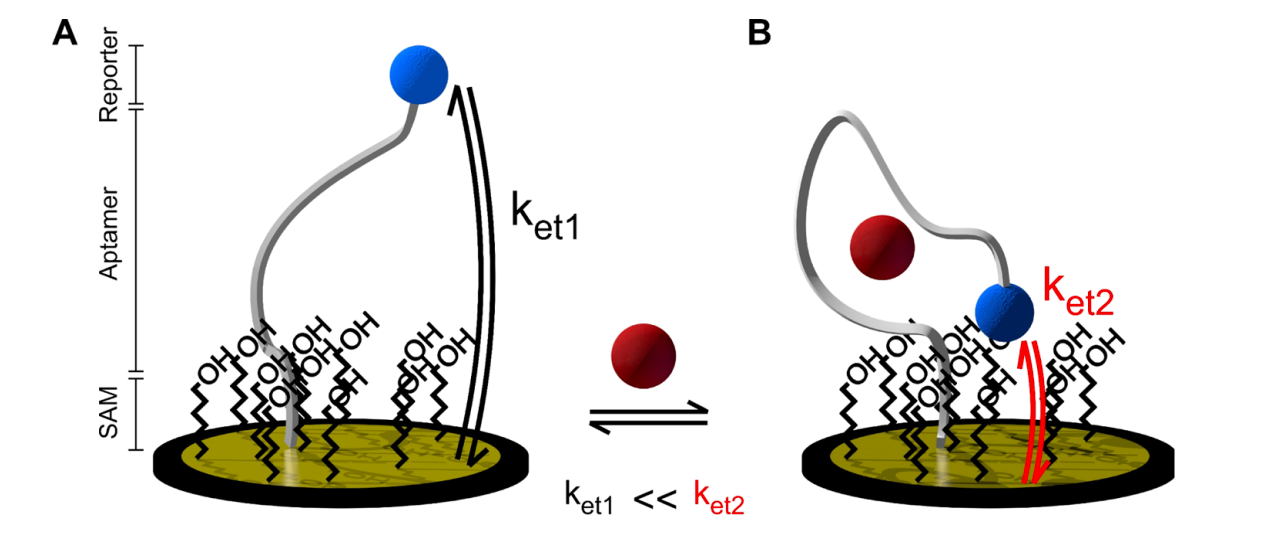
\includegraphics[width = 1.0\textwidth]{img/aptamerdiagram2.png}
    \caption{Aptamer Electron transfer rate. Increases due to Target binding to the Aptamer.\cite{arroyo2018subsecond}}
    \label{aptamerrate}
\end{figure}
Target ([T]) binding to the Aptamer ([A]), forms the aptamer-ligand complex ([AT]) as shown in the following chemical reaction:
\begin{align}
\cee{[A] + [T]  &<=> [AT]} 
\end{align}
The binding rate of the target to the aptamer is $k_{on}$ and the off-binding rate of the target to the aptamer is $k_{off}$. Assuming the system is in equilibrium, the rate of the forward reaction is equal to the rate of the backward reaction:
\begin{equation}
k_{on}[A][T] = k_{off}[AT]
\end{equation}
Using the conservation of mass for the total aptamer concentrations:
\begin{equation}
[A_{0}] = [A] + [AT]
\end{equation}
Faradaic reduction of the methylene blue reporter to leucomethylene blue occurs during chronoamperometric detection
 \cite{zhan1990mechanisms}:
\begin{align}
\cee{MB^{+} + 2e^{-} + H^{+}  &-> LMB} 
\end{align}
Electron transfer empirically follows a first order rate reaction \cite{bard1983electrochemical, forster1994electrochemistry}. Therefore the output current follows an exponential decay.
% $$ k_{ET} = -\frac{d[e^{-}]}{dt} $$
% $$ \therefore [e^{-}] = e^{-k_{ET}t} $$

\subsection{Chronoamperometric Signal}
Upon a step wave excitation in potential during chronoamperometry, the output current is a sum of exponential decay signals \cite{arroyo2018subsecond}, one due to the bound aptamer, and another due to the unbound aptamer, with the relative contributions of the exponential decays to be equal to the concentrations of the bound and unbound aptamers respectively. The two exponential decay components are likely to be a distribution, centered at the mean average value. Modelling the rate constants 'k' as a probability distribution would more physically represent the physical scenario.
$$ \frac{i}{nFA} = [AT]e^{-k_{AT}t} + [A]e^{-k_{A}t} $$
Deriving the expressions for the concentrations of the bound and unbound aptamer configurations as functions of the total aptamer concentration - we use equations (2) and (3) to derive [AT]:
$$ [AT] = \frac{k_{on}[T][A_{0}-AT]}{k_{off}} $$
$$ [AT] = \frac{k_{on}[T][A_{0}]}{k_{off}} - \frac{k_{on}[T][AT]}{k_{off}} $$
$$ [AT](1+\frac{k_{on}[T]}{k_{off}}) = \frac{k_{on}[T][A_{0}]}{k_{off}} $$
$$  [AT] = \frac{k_{on}[T]}{k_{off}+k_{on}[T]}[A_{0}] $$
Using a similar method, we can get an expression for [A], concentration of the unbound aptamer. Alternatively, we can calculate [A] using the conservation of mass formula, where [A] = [$A_{0}$]-[AT]:
$$ [A] = \frac{k_{off}}{k_{off}+k_{on}[T]}[A_{0}] $$
Final equation for the output current:\\\\
\begin{equation}
\frac{i}{nFA} = \frac{k_{on}[T]}{k_{on}[T]+k_{off}}e^{-k_{AT}t} + \frac{k_{off}}{k_{on}[T]+k_{off}}e^{-k_{A}t}
\end{equation}
\clearpage
\section{Aptamer Modelling Code} \label{app:apt_mod}
\subsection{Multiexponential Rate Extraction Code}
\lstinputlisting{Code/Rate_res_testing.m}
\newpage
\subsection{Numerical Inverse Laplace Solver}
\lstinputlisting{Code/iLaplace.m}
\newpage
\subsection{Coarse-grained Aptamer Modelling}
\lstinputlisting{Code/Chain_sim_bound_unbound_v3.m}
\newpage
\subsection{Probability from DNA length Model}
\lstinputlisting{Code/Electron_transfer_FINAL.m}
\newpage

%=====================================================================================
\section{Risk Assessment}
% \begin{table}[H]
%     \centering
    \begin{longtable}{|p{.1\textwidth}|p{.1\textwidth}|p{.1\textwidth}|p{.1\textwidth}|p{.1\textwidth}|p{.1\textwidth}|p{.08\textwidth}|p{.13\textwidth}|}\hline
        \textbf{Hazard} & \textbf{Risk} & \textbf{Likelihood} & \textbf{Severity} & \textbf{Risk rating} & \textbf{Mitigation} & \textbf{Revised risk} & \textbf{Contingency }\\ \hline
        
        Lab unavailability & Unable to test blood samples & 2 & 3 & 6 & \textit{N/A} & \textit{N/A} & Move to literature based research on how blood sampling results may differ \\ \hline
        
        Chemical shortages e.g enzyme & Cannot test new markers & 4 & 3 & 12 & \textit{N/A} & \textit{N/A} & Use pre-fabricated sensors where available or else move to literature based research \\ \hline
        
        Inadequate sensitivity (detection falls in desired detection range) & Unable to produce sufficient calibration curves & 1 & 4 & 4 & \textit{N/A} & \textit{N/A} & Produce curves until detection limit, use literature to investigate how behaviour is expected to progress beyond experimented concentrations \\ \hline
        
        Faulty equipment & Unable to conduct electrochemical tests & 3 & 5 & 15 & \textit{N/A} & \textit{N/A} & Borrow or purchase replacements\\ \hline
        
        Sodium lactate & Can cause skin and eye irritation, irritation of digestive and respiratory tract. & 2 & 3 & 6 & Wear gloves and face masks, avoid prolonged exposure. Flush eyes/skin upon contact & 1 & \textit{N/A}\\ \hline
        
        Sodium nitrite NaNO3 & Toxic if swallowed, serious eye irritation & 2 & 4 & 8 & Do not eat in lab, wear gloves and mask. Immediately seek medical attention if swallowed. & 3 & \textit{N/A}\\ \hline
        
        \pagebreak
        
        Hydrogen Peroxide solution H2O2 &  Can cause severe burn injuries on contact with skin or eyes. & 2 & 4 & 8 & Diluted samples used. Use gloves and seek medical attention in case of contact & 3 & \textit{N/A}\\ \hline
        
        
        Electrical equipment & Can overheat and malfunction. & 2 & 4 & 6 & Turn off appliances when not in use. If overheating, terminate experiments and continue after a break where possible. & 3 & \textit{N/A}\\ \hline
        
        Chemical spills & Can come in to contact with live wires causing explosions. & 2 & 4 & 8 & Keep wet experiments away from live electrical appliances, use insulated wires and small volumes of liquid. Clean any spills immediately & 3 & \textit{N/A}\\ \hline
    \end{longtable}
% \end{table}



%=====================================================================================

\end{appendices}